\documentclass[notes]{subfiles}
\begin{document}
	\addcontentsline{toc}{section}{4.4 -  Inflection Points \& Second Derivatives}
	\refstepcounter{section}
	\fancyhead[RO,LE]{\bfseries  \large \nameref{cs44}} 
	\fancyhead[LO,RE]{\bfseries  \currentname}
	\fancyfoot[C]{{}}
	\fancyfoot[RO,LE]{\large \thepage}	%Footer on Right \thepage is pagenumber
	\fancyfoot[LO,RE]{\large Chapter 4.4}

\section*{Inflection Points \& Second Derivatives}\label{cs44}
	\subsection*{Definitions}
		\begin{defn}[Inflection Point] 
			An \textbf{inflection point} is the point on the graph of a function where \showto{ins}{\fbox{the function changes}\\ \fbox{concavity}.}\showto{st}{\blank{2}\\[15pt] \blank{3}.}
		\end{defn}
			\vs{.25}
			
		An inflection point gives the point of \showto{ins}{\fbox{most/least rapid}}\showto{st}{\blank{3}} change of the function.
			\vs{.25}
			
		\begin{thm}[Properties of the Second Derivative]
			Let $f(x)$ be a twice-differentiable function defined on input interval $[a,b]$, with $a < c < b$.  \\$ $ \\
				\tabitem $f$ has an inflection point at $x = c$ if and only if \showto{ins}{\fbox{$f''(c) = 0$ and changes sign}\\}\showto{st}{\blank{2}.\\[15pt]}
				\tabitem If $f''(c)$ is positive, then \showto{ins}{\fbox{$f$ is concave up}\\}\showto{st}{\blank{4}.\\[15pt]}
				\tabitem If $f''(c)$ is positive, then \showto{ins}{\fbox{$f'$ is increasing}\\}\showto{st}{\blank{4}.\\[15pt]}
				\tabitem If $f''(c)$ is negative, then \showto{ins}{\fbox{$f$ is concave down}\\}\showto{st}{\blank{4}.\\[15pt]}
				\tabitem If $f''(c)$ is negative, then \showto{ins}{\fbox{$f'$ is decreasing}\\}\showto{st}{\blank{4}.\\[15pt]}
				
		\end{thm}
			\vs{.25}
		\begin{thm}[Second Derivative Test]
			Let $f(x)$ be a twice-differentiable function defined on input interval $[a,b]$, with $a < c < b$.\\$ $\\
					\tabitem \showto{ins}{\fbox{If $f'(c) = 0$ and $f''(c) > 0$, then $f$ has a relative minimum at $c$}\\}\showto{st}{\blank{6}.\\[15pt]}
					\tabitem \showto{ins}{\fbox{If $f'(c) = 0$ and $f''(c) < 0$, then $f$ has a relative maximum at $c$}}\showto{st}{\blank{6}.}
		\end{thm}
			\vs{.25}
			\newpage
			
	\subsection*{Examples}
		\begin{ex} 
			The percentage of people living in California in 2007 who were born in the state can be modeled as
			\[P(x) = -0.0016x^3 + 0.224x^2-10.577x + 204.8\text{ percent}\]
			where $x$ is the age of the resident.
			\begin{enumerate}[(a)]
				\item Find the inflection point of the function $P$.
					\vs{1.5}
					
				\item Give a sentence of interpretation for the age between 20 and 70 at which the percentage of California residents who were born in the state was decreasing least rapidly.
					\vs{1}
					
			\end{enumerate}
		\end{ex}
		
		\begin{ex} For the function
			\[f(t)=-2.1t^2 + 7t\]
			\begin{enumerate}[(a)]
				\item Write the first and second derivative.
					\vs{2}
					
				\item Identify any inflection points, and label them as the point of \emph{least rapid} or \emph{most rapid} change.
					\vs{1.5}
			\end{enumerate}
		\end{ex}
			\newpage
			
		\begin{ex} 
			The percentage of new material that an average college student will retain after studying for $t$ hours without a break can be modeled as
			\[p(t) = \frac{83}{1+5.94e^{-0.969t}}\text{ percent}\]
			\begin{enumerate}[(a)]
				\item Find when the retention rate is increasing most rapidly.
					\vs{1.5}
					
				\item Determine the rate of change of retention as well as the percentage of retention at the input found in item (a).
					\vs{1}
					
				\item Describe the difference between the direction of $p$ and $p'$ to the right of the input found in item (a).
					\vs{1.5}
					
				\item Explain what happens to the student's retention rate after the input found in item (a).
					\vs{1}
					
			\end{enumerate}
		\end{ex}
			\newpage

		\begin{ex} For the function
			\[g(s) = 32s^3 + 2.1s^2 + 7s\]
			\begin{enumerate}[(a)]
				\item Write the first and second derivative.
					\vs{1.5}
					
				\item Identify any inflection points, and label them as the point of \emph{least rapid} or \emph{most rapid} change.
					\vs{1}
			\end{enumerate}
		\end{ex}
		
		\begin{ex} For the function
			\[h(x) = e^{3x} - \ln 3x\]
			\begin{enumerate}[(a)]
				\item Write the first and second derivative.
					\vs{1.5}
					
				\item Identify any inflection points, and label them as the point of \emph{least rapid} or \emph{most rapid} change.
					\vs{1}
					
			\end{enumerate}
		\end{ex}
			\newpage
			
		\begin{ex} For the function
			\[k(t) =  \frac{16}{1+2.1e^{3.9t}}\]
			\begin{enumerate}[(a)]
				\item Write the first and second derivative.
					\vs{2}
					
				\item Identify any inflection points, and label them as the point of \emph{least rapid} or \emph{most rapid} change.
					\vs{1}
					
			\end{enumerate}
		\end{ex}
		
		\begin{ex} For the function
			\[f(x) = -x^3+12x^2 + 36x + 45\]
			\begin{enumerate}[(a)]
				\item Write the first and second derivative.
					\vs{1}
					
				\item Identify any inflection points, and label them as the point of \emph{least rapid} or \emph{most rapid} change.
					\vs{1}
					
			\end{enumerate}
		\end{ex}
			\newpage
			
		\begin{ex} 
			The table below shows the monthly revenue levels associated with various monthly levels of advertising by a furniture store.
				\begin{center}
					{\renewcommand{\arraystretch}{1.2}
					\begin{tabular}{|c|c|c|c|c|c|c|c|}\hline
					\textbf{Advertising} (in hundreds of dollars) & 1 & 4 & 7 & 10 & 13 & 16 & 19\\ \hline
					\textbf{Revenue} (in thousands of dollars) & 114 & 210 & 265 & 299 & 338 & 449 & 632\\ \hline
					\end{tabular}
					}
				\end{center}
			\begin{enumerate}[(a)]
				\item Find the \textbf{complete} cubic model $R(x)$ for the data (do not align the input).
					\vs{1}
					
				\item Write the \textbf{complete} rate of change model for $R(x)$.
					\vs{1.5}
					
				\item Find $R''(x)$.
					\vs{1}
					
				\item Find the inflection point of $R(x)$ on the interval $[0,19]$.  Round both coordinates to the hundredths place and be sure to label them with units.
					\vs{1}
					
				\item Find the rate of change at the inflection point.  Round to the hundredths place and include units in your answer.
					\vs{1}
					
			\end{enumerate}
		\end{ex}
			\newpage
			
		\begin{ex}
			Consider the following graphs:
				\begin{center}
					{\renewcommand{\arraystretch}{1.2}
					\begin{tabular}{cccccc}
						\textbf{A} & 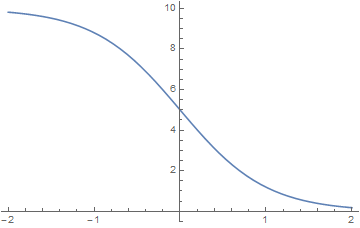
\includegraphics[scale=.3]{./img/44-1.png} & \textbf{B} &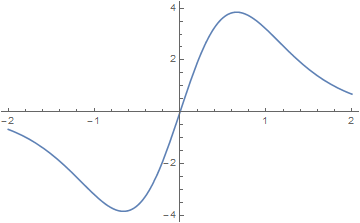
\includegraphics[scale=.3]{./img/44-3.png}&\textbf{C}&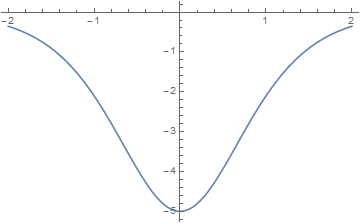
\includegraphics[scale=.3]{./img/44-2.png}
					\end{tabular}
					}
				\end{center}
				\begin{enumerate}[(a)]
					\item Write ``True'' or ``False'' to the left of the following statements:
						\begin{center}
							\begin{tabular}{ll}
								& \\ &\\
							\makebox[1in]{\hrulefill} & The graph of the derivative of \textbf{A} will have no $x-$intercepts.\\
								& \\ &\\
							\makebox[1in]{\hrulefill} & The graph of the derivative of \textbf{B} will have exactly one $x-$intercept.\\
								&\\ &\\
							\makebox[1in]{\hrulefill} & The graph of the second derivative of \textbf{C} will have exactly two $x-$intercepts.\\
								&\\ &\\
							\makebox[1in]{\hrulefill} & The graph of the second derivative of \textbf{A} will always be negative.\\
								&\\ &\\
							\end{tabular}
						\end{center}
					\item Which of the following describes the relationship between these three graphs?  \emph{Mark an X to the left of your choice}.
						\begin{center}
							\begin{tabular}{ll}
								& \\ & \\
							\makebox[1in]{\hrulefill} & \textbf{B} is $f(x)$, \textbf{C} is $f'(x)$, and \textbf{A} is $f''(x)$.\\
								&\\ &\\
							\makebox[1in]{\hrulefill} & \textbf{A} is $f(x)$, \textbf{C} is $f'(x)$, and \textbf{B} is $f''(x)$.\\
								&\\ &\\
							\makebox[1in]{\hrulefill} & \textbf{C} is $f(x)$, \textbf{A} is $f'(x)$, and \textbf{B} is $f''(x)$.\\  
								&\\ &\\
							\makebox[1in]{\hrulefill} & \textbf{B} is $f(x)$, \textbf{A} is $f'(x)$, and \textbf{C} is $f''(x)$.\\  
							\end{tabular}
						\end{center}
				\end{enumerate}
			\end{ex}
	\clearpage
\end{document}